% !TEX TS-program = pdflatex
% !TEX encoding = UTF-8 Unicode
\documentclass{book}
% !TEX encoding = UTF-8 Unicode
\usepackage{dhucs}
\usepackage{dhucs-trivcj}
\usepackage{geometry}
%\geometry{left=40mm,right=40mm,top=30mm,bottom=40mm}

\usepackage{times} %Times New Roman font

\usepackage{setspace} %줄간격 package
\onehalfspacing

\usepackage[dvipdfmx]{graphicx}
\graphicspath{{./Figure/}}

\usepackage[nottoc]{tocbibind}

\usepackage{amsmath,amssymb}

\usepackage{enumitem}%좀 더 fancy한 itemize를 위한 패키지

\usepackage{changepage}%문단을 들여쓰기 하기 위한 패키지

\usepackage{subcaption}%sub figure를 위한 패키지

\usepackage{array}%표를 그리기 위한 패키지

\renewcommand{\arraystretch}{1.2} % 행 간 간격을 1.5배로 설정
\setlength{\tabcolsep}{8pt} % 열 간 간격을 10pt로 설정

%\usepackage[sorting=none, style=science]{biblatex}
%\bibliography{reference}

\usepackage{fancyhdr} %머릿글 꼬릿글 설정 package

\usepackage{pict2e} % for drawing picture

\usepackage{here}
\usepackage{url}
\usepackage{mathrsfs}
\usepackage[version=3]{mhchem}
\usepackage{indentfirst}\setlength\parindent{2em}
\usepackage{color}


\usepackage{kotex}
\usepackage{CJKutf8}

%\newenvironment{m}{\begin{eqnarray}}{\end{eqnarray}}
%\setcounter{tocdepth}{2}

%\def\theequation{\arabic{chapter}.\arabic{section}.\arabic{equation}}
%\makeatletter
%\makeatother

%\def\thline{\noalign{\hrule height 1pt}}
%\def\tvline{\vrule width 1pt} 

%\renewcommand{\appendixname}{Appendix}
%\setlength{\textwidth}{\fullwidth}
%\setlength{\evensidemargin}{\oddsidemargin}



\title{Coulomb Dissociation of Borromean Nuclei ${}^{17}B$}
\author{Hyeji Lee}
\date{\today}

\begin{document}
\frontmatter
\maketitle
\pagenumbering{arabic}
%\pagenumbering{romanw}
\clearpage

\thispagestyle{empty}

\clearpage

\thispagestyle{empty}
\chapter*{Abstract}
Neutron-rich isotopes have received much attraction in recent years due to its structural properties such as neutron halo: one or two neutrons in the nucleus are weakly bound so that they are spatially extended far from the core nucleus. Borromean nuclei are particularly interesting due to the two-neutron halo structure. The Borromean nucleus is a bound three-body system, where any of its two-body subsystems are unbound. Experimental data of 2n halo structure has been reported for 6He, 11Li, and 19B. These 2n halo nuclei are possible to have a dineutron correlation, a spatially compact neutron pair, and the recent Coulomb dissociation of 19B revealed the dineutron in 19B. [1] We focus on 17B, which is also considered as a 2n halo nucleus. 17B is the core of the 2n halo nucleus 19B but 17B itself is the 2n halo nucleus. Investigating a dineutron correlation in the 17B will gives us a critical information about multi-neutron halo structure in neutron-rich isotopes.
To investigate the dineutron correlation at the 17B, the experimental measurement using Coulomb dissociation was performed at SAMURAI (Superconducting Analyser for MUlti particles from RAdio Isotope beams) spectrometer in RIBF (Radioactive Isotope Beam Factory), RIKEN. A 48Ca primary beam accelerated to 345 MeV per nucleon was incident on a primary Be target to produce a 17B secondary beam. The generated secondary beam was separated and identified by BigRIPS fragment separator and was incident into a secondary Pb target where 17B is dissociated into 15B and two neutrons. The charged fragment 15B was detected by the SAMURAI spectrometer, while the two neutrons were detected by the neutron detectors NEBULA to measure Coulomb dissociation exclusive cross section. In this poster, we report the current analysis statue.

\clearpage
\tableofcontents
%\listoffigures
%\listoftables


\mainmatter
\pagenumbering{arabic}

%\chapter{Introduction}
최근 몇년간, 가속기를 이용한 핵물리 실험이 급진적으로 발전함에 따라, 불안정 핵에 대한 연구가 급격하게 진행되었다. 특히 자연에서는 존재하지 않는 beta stability에서 먼, 원자핵의 존재 한계에 가까운 드립라인 핵에 대한 연구가 가능하게 되었다. 특히 양성자의 수보다 중성자의 수가 훨씬 많은 중성자 과잉 핵자에서는 안정 핵자에서는 볼 수 없는 특이한 현상들을 관찰 할 수 있는데, 중성자 헤일로가 대표적이다. \\
\indent 중성자 헤일로는 하나 또는 두개의 중성자가 코어로부터 공간적으로 멀리 떨어져있는 핵자다. 헤일로 중성자는 코어로부터 매우 약하게 속박되어 있고, 낮은 centrifugal barrier 를 갖고있는 낮은 궤도 각 운동량 l=0 or 1를 갖고 있는 것이 특징이다. 이러한 특징으로 기인하는 중성자 헤일로 핵의 고유한 특징은 1MeV 이하의 아주 작은 중성자 분리 에너지 (안정핵은 보통 8MeV이다)와 주변핵자에 비해 매우 큰 반경, 그리고 Soft E1 Excitation이 있다.
그림1.1\ref{Nuclear chart}를 보면 원자번호 1부터 12까지의 핵자표가 있고, 원으로 표시된 핵자가 헤일로 핵자이다. 하나의 원은 1 중성자 헤일로, 2개의 원은 2중성자 헤일로이다. 지금까지 발견된 2중성자 헤일로는 6He, 11Li, 14Be, 17B, 19B, 22C로 

Over recent years, The study of neutron-rich nuclei has garnered increasing attention within the field of nuclear physics, providing invaluable insights into the fundamental forces and interactions that govern atomic nuclei. Characterized by an excess of neutrons compared to stable isotopes, these nuclei serve as a compelling laboratory for investigating phenomena that transcend conventional nuclear models. One particularly intriguing subclass is that of 2-neutron halo nuclei, which feature an extended halo of two loosely bound neutrons.\cite{tanihata} This thesis aims to delve deeper into the enigmatic properties and behaviors of 2-neutron halo nuclei, contributing to our broader comprehension of neutron-rich systems.

\begin{figure}[h]
    \centering
    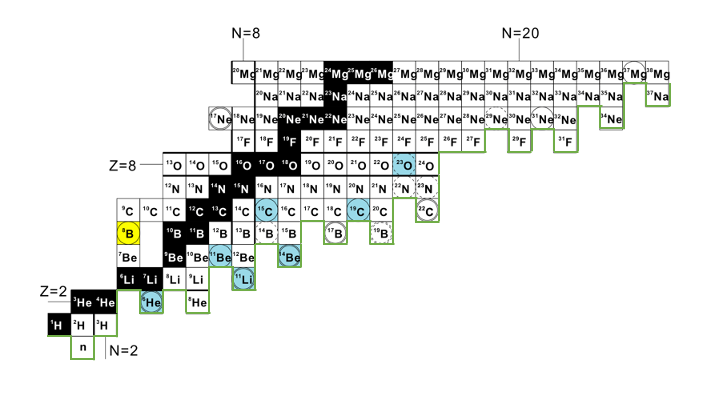
\includegraphics[width=14cm]{nuclear_chart.png}
    \caption{Nuclear Chart}
    \label{Nuclear chart}
\end{figure}

\begin{figure}
    \centering
    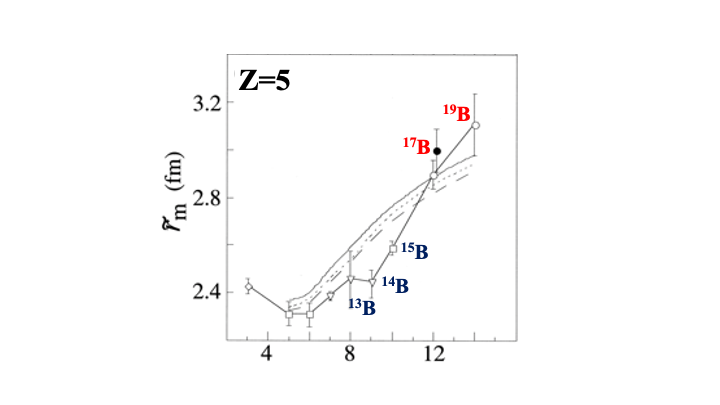
\includegraphics[width=14cm]{Radius_of_boron.png}
    \caption{Caption}
    \label{fig:enter-label}
\end{figure}
2 중성자 헤일로로 알 수 있는 것은 dineutron에 대한 연구이다. 

본 논문에서는 납 타겟을 이용하여 17B를 






\backmatter

 

\end{document}
